\clearpage

\section{Cantorin kosinta}

Kolossi Cantor on silminnähden rakastunut. Hän on jo pitkään palvonut toista jättiä, Ada Lovelacea. Cantor on päättänyt ottaa seuraavan askeleen heidän suhteessaan. Hän on päättänyt kosia Adaa. Tätä varten Cantorin täytyy tilata sormus. 


Adalla valtavat neliönmuotoiset sormet. Tämän takia sormus täytyy tilata mittatilaustyönä. Onneksi Cantor tietää, että Adan nimettömän leveys on $2,5 \ \text{m}$.


Kuinka suuri täytyy ympyränmuotoisen sormuksen ympärysmitan olla?


\begin{figure}[h]
    \begin{subfigure}{.5\textwidth}
        \centering
        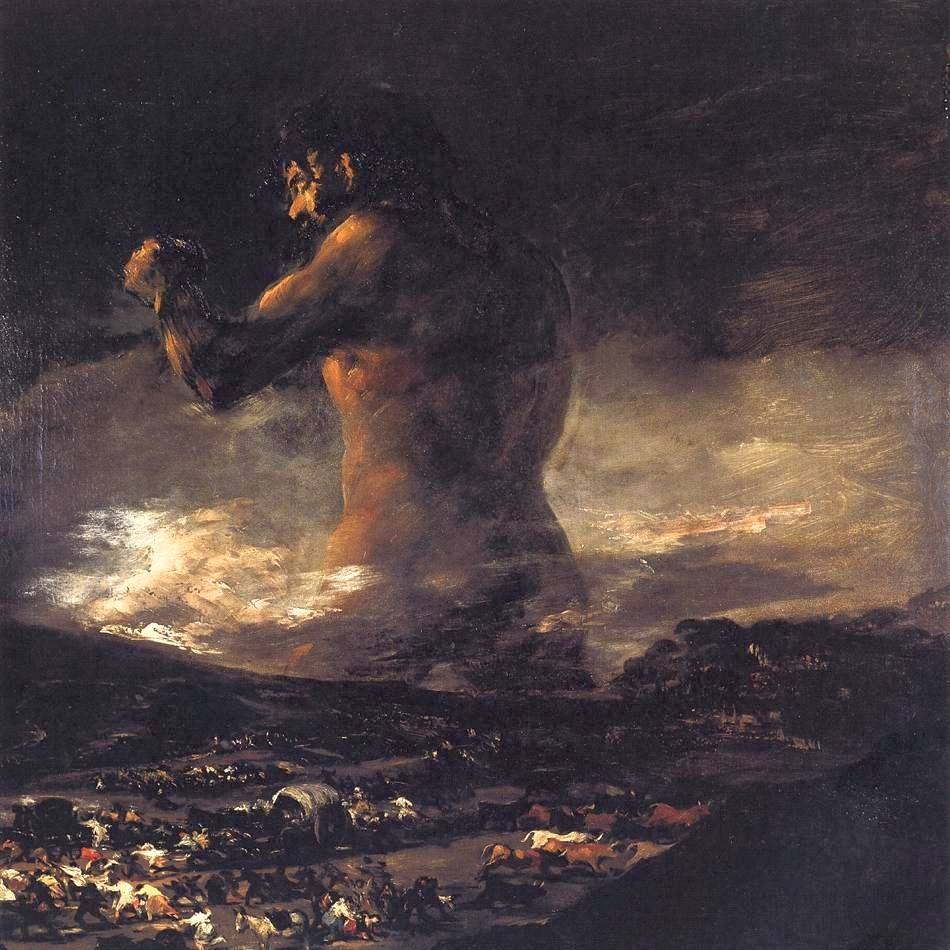
\includegraphics[width=.9\linewidth]{kuvat/cantor_jättiläinen.jpg}
        \caption*{Rakastunut kolossi Cantor}
  \end{subfigure}%
  \begin{subfigure}{.5\textwidth}
  \centering
    \includegraphics[width=.9\linewidth]{kuvat/cantorin_ympyrä.png}
    \caption*{Poikkileikkaus Adan sormesta}
  \end{subfigure}
\end{figure}
